\documentclass[tikz,border=2mm]{standalone}
\usepackage{tikz}
\usetikzlibrary{shapes.geometric, arrows, shapes.gates.logic.US, calc}

\tikzstyle{arrow} = [thick,->,>=stealth]

\begin{document}
    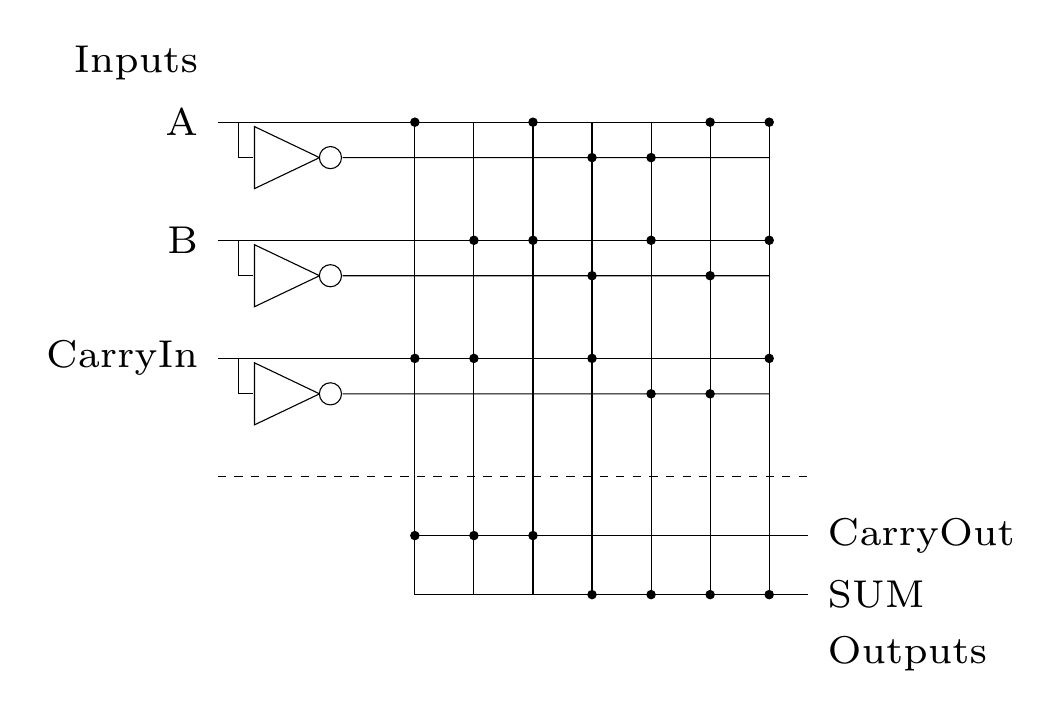
\begin{tikzpicture}[node distance=2cm, scale=1.5, every node/.style={scale=2}]

        % Inputs
        \node at (0,0.5) [left] (A) {\scriptsize Inputs};
        
        % A input with not gate
        \node at (0,0) [left] (A) {\scriptsize A};
        \draw (0, 0) -- (4.67,0);
        \node at (0.5,-0.3) [not gate US,draw](not) {};
        \draw (0.18, 0) |- (not.input);
        \draw (not.output) -- (4.67,-0.3);
        
        % B input with not gate
        \node at (0,-1) [left] (B) {\scriptsize B};
        \draw (0, -1) -- (4.67,-1);
        \node at (0.5,-1.3) [not gate US,draw](not) {};
        \draw (0.18, -1) |- (not.input);
        \draw (not.output) -- (4.67,-1.3);
        
        % CarryIn input with not gate
        \node at (0,-2) [left] (B) {\scriptsize CarryIn};
        \draw (0, -2) -- (4.67,-2);
        \node at (0.5,-2.3) [not gate US,draw](not) {};
        \draw (0.18, -2) |- (not.input);
        \draw (not.output) -- (4.67,-2.3);
        
        % AND plane
        \draw [dashed] (0, -3) -- (5, -3);
        
        % AND Connections
        % A AND CarryIn
        \draw (1.67, 0) -- (1.67, -4);
        \filldraw[black] (1.67, -0) circle (1pt);
        \filldraw[black] (1.67, -2) circle (1pt);
        
        % B AND CarryIn
        \draw (2.17, 0) |- (2.17,-4);
        \filldraw[black] (2.17, -1) circle (1pt);
        \filldraw[black] (2.17, -2) circle (1pt);
        
        % A AND B
        \draw (2.67, 0) |- (2.67,-4);
        \filldraw[black] (2.67, -0) circle (1pt);
        \filldraw[black] (2.67, -1) circle (1pt);
        
        % NOT(A) AND NOT(B) AND CarryIn
        \draw (3.17, 0) |- (3.17,-4);
        \filldraw[black] (3.17, -0.3) circle (1pt);
        \filldraw[black] (3.17, -1.3) circle (1pt);
        \filldraw[black] (3.17, -2) circle (1pt);
        
        %  NOT(A) AND B AND NOT(CarryIn)
        \draw (3.67, 0) |- (3.67,-4);
        \filldraw[black] (3.67, -0.3) circle (1pt);
        \filldraw[black] (3.67, -1) circle (1pt);
        \filldraw[black] (3.67, -2.3) circle (1pt);
        
        %  A AND NOT(B) AND NOT(CarryIn)
        \draw (4.17, 0) |- (4.17,-4);
        \filldraw[black] (4.17, -0) circle (1pt);
        \filldraw[black] (4.17, -1.3) circle (1pt);
        \filldraw[black] (4.17, -2.3) circle (1pt);
        
        %  A AND B AND CarryIn
        \draw (4.67, 0) |- (4.67,-4);
        \filldraw[black] (4.67, -0) circle (1pt);
        \filldraw[black] (4.67, -1) circle (1pt);
        \filldraw[black] (4.67, -2) circle (1pt);
        
        % OR Connections
        \node at (5,-4.5) [right] (A) {\scriptsize Outputs};
        \node at (5,-3.5) [right] (B) {\scriptsize CarryOut};
        \node at (5,-4) [right] (B) {\scriptsize SUM};
        \draw (1.67,-3.5) |- (5,-3.5);
        \draw (1.67,-4) |- (5,-4);
        \filldraw[black] (1.67, -3.5) circle (1pt);
        \filldraw[black] (2.17, -3.5) circle (1pt);
        \filldraw[black] (2.67, -3.5) circle (1pt);
        \filldraw[black] (3.17, -4) circle (1pt);
        \filldraw[black] (3.67, -4) circle (1pt);
        \filldraw[black] (4.17, -4) circle (1pt);
        \filldraw[black] (4.67, -4) circle (1pt);
            
        
    \end{tikzpicture}
\end{document}
